
\documentclass[]{article}
% packages
\usepackage{../../cs70}
\usepackage{../../markup}
\usepackage{enumerate}
\usepackage{hyperref}
%% \usepackage{framed}
%% \usepackage{MnSymbol}
%% \usepackage{epstopdf}
\usepackage{color}
\usepackage[]{amsmath}
\usepackage{cancel}
%% \usepackage{graphicx}
%% \usepackage{amssymb}
%% \usepackage{parskip}
%% \usepackage{rotating}
%% \usepackage{float}
%% \usepackage{multirow}
%% \usepackage{subcaption}
%% \usepackage{indentfirst}
%% \usepackage[left=1.5in, right=1.0in, top=1.0in, bottom=1.0in]{geometry}

\newtheorem{Definition}{Definition}
\newtheorem{Lemma}{Lemma}
\newtheorem{Proof}{Proof}
\newtheorem{Theorem}{Theorem}

\newif\ifsolutions
\newif\ifmotivation
\motivationtrue
\motivationfalse
\solutionstrue
%\solutionsfalse %flag for solutions

\renewcommand{\answer}[1]{{\color{mydarkblue}\textbf{Solution:}#1}}
\definecolor{mydarkblue}{rgb}{0,0.25,1}

\def \exx {\mathbb{E}}
\def\title{Homework 12}

\begin{document}

\maketitle
\config{hwnum}{12}
\config{homework-due}{04/21/2014 13:00}
\config{grades-due}{04/28/2014 13:00}
\vspace{0.5em}
{\Large{\textbf{This homework is due April 21 2014, at 12:00 noon.}}}

\begin{qunlist}

\qns{Independent Random Variables}\\
Find four random variables taking values in $\{-1,1\}$ so that any three are independent but all four are not.

\ifsolutions{ \answer{
Let $X_1,X_2,X_3,X_4$ be i.i.d random variables with $P(X_i=1)=P(X_i=-1)=1/2$. Let $X_4=X_1X_2X_3$. Check that $X_1,X_2,X_3,X_4$ are four random variables such that any three are independent but all four are not. For example, they are not all independent because
\[
P(X_1=1,X_2=1,X_3=1,X_4=1)=1/8 \neq
P(X_1=1)P(X_2=1)P(X_3=1)P(X_4=1)
\]
}}
\fi

\qns{Expectation Basics} \\ For discrete random variables $X$ and $Y$:
\begin{enumerate}[a)]

\qpart
\item Show that for constants $c$ and $d$, $\mathbb{E}[cX + dY] = c\mathbb{E}[X] + d \mathbb{E}[Y]$.

\ifsolutions{ \answer{ Beginning with the left-hand-side:
		\begin{align*}
		\mathbb{E}[cX + dY] & = \sum_x \sum_y (cx+dy) \mathbb{P}(x,y) & \text{definition of expectation} \\
		& = c\sum_x \sum_y x \mathbb{P}(x,y) + d\sum_x \sum_y y \mathbb{P}(x,y) & \text{expand and break up the sum into two parts} \\
		& = c \sum_x x \sum_y \mathbb{P}(x,y) + d \sum_y y \sum_x \mathbb{P}(x,y) & \text{reorder terms that depend on $x$ or $y$} \\
		& = c\sum_x x \mathbb{P}(x) + d\sum_y y \mathbb{P}(y) & \text{marginalize over $y$ in the first term and $x$ in the second term} \\
		& = c\mathbb{E}[X] + d \mathbb{E}[Y]. & \text{arrive at the definition of expectation for $X$ and $Y$}
		\end{align*}

One of the key steps was using the fact that
\[ \sum_{y} \mathbb{P}(x,y) = \mathbb{P}(x). \]

This is often phrased as ``marginalizing out'' a variable, to retain only the variables of interest.  In this case we are marginalizing out $y$ and retaining only the probability of $x$.
}}
\fi


\qpart
\item Show that $\mathbb{E}[\min(X,Y)] + \mathbb{E}[\max(X,Y)]  = \mathbb{E}[X] + \mathbb{E}[Y]$.

\ifsolutions{ \answer {
\begin{align*}
\mathbb{E}[\min(X,Y)] + \mathbb{E}[\max(X,Y)] & =  \mathbb{E}[\min(X,Y) + \max(X,Y)] &  \text{By linearity of expectation} \\ & = \mathbb{E}[X + Y] \\ & = \mathbb{E}[X] + \mathbb{E}[Y] & \text{By linearity of expectation}
\end{align*}

}}
\fi


%-show that if $X$ and $Y$ are independent discrete random variables, then \[\mathbb{E}[XY] = \mathbb{E}[X] \mathbb{E}[Y].\]  Does this property imply independence?


\end{enumerate}

\qns{Variance of Random Variables} %Independent R.V.s}

The variance of a random variable tells us information about how far the random variable is spread outside its expectation. For this problem, we will use the definition $Var[X] = \exx[X^2] - \exx[X]^2$.  We already know how to compute the expectation of a sum of random variables because expectation is linear ($\mathbb{E}[X+Y] = \mathbb{E}[X] + \mathbb{E}[Y]$). In this problem, we will compute the variance of $Z$, where $Z$ is a sum of random variables:
\[ Z = \sum_{i=1}^n X_i \]
%For the rest of the problem, we consider a set of random variables
and $X_1, X_2, \cdots, X_n$ are pair-wise independent (this means $\forall{i \neq} j $ Pr$[X_i = a \cap X_j = b] = Pr[X_i = a]Pr[X_j = b]$ ).
\begin{enumerate}[a)]
\qpart
\item In order to compute the variance of the sum of these random variables, first  prove the following lemma: \\ \textbf{Lemma:} If $X$ and $Y$ are independent random variables, then $\exx[XY] = \exx[X] \exx[Y]$. \\  
(Hint: Let $\mathcal{X}$ be the set of all possible values of $X$ and let $\mathcal{Y}$ be the set of all possible values of $Y$. Now use the definition of expectation, $\exx[XY] = \sum\limits_{x \in \mathcal{X}} \sum\limits_{y \in \mathcal{Y}} xy \cdot Pr[X=x \cap Y = y]$).
\ifsolutions{ \answer {
We start with the hint. \\  $\exx[XY] = \sum\limits_{x \in \mathcal{X}} \sum\limits_{y \in \mathcal{Y}} xy \cdot Pr[X=x \cap Y = y] \\ = \sum\limits_{x \in \mathcal{X}} \sum\limits_{y \in \mathcal{Y}} xy \cdot Pr[X=x] Pr[Y = y]$ Because $X$ and $Y$ are independent $\\ = \sum\limits_{x \in \mathcal{X}} Pr[X=x] \cdot x \sum\limits_{y \in \mathcal{Y}} y \cdot Pr[Y = y]$ Because $x$ does not change in the inner summation. $\\ = \sum\limits_{x \in \mathcal{X}} Pr[X=x] \cdot x \exx[Y]$ By definition of expectation $\\ = \exx[Y] \cdot \sum\limits_{x \in \mathcal{X}} Pr[X=x] \cdot x = \exx[Y]\exx[X]$
}}
\fi

\qpart
\item
%Let $X$ be a sum of pair-wise independent random variables. So $X = \sum\nolimits_{i=1}^n X_i$. We wish to solve for $Var[X]$. We break this into a few steps. First note that $Var[X] = \exx[X^2] - \exx[X]^2$. \\ 
Prove that $\exx[Z^2] = \sum\nolimits_{i=1}^n \exx[X_i^2] + \sum_{i=1}^n \sum_{j \neq i} \exx[X_iX_j]$. \\ 
(Hint: 
What happens when you expand out $(X_1 + X_2 + \cdots X_n)^2$?)
\ifsolutions{ \answer {
We start with the hint, we see that $Z = (X_1 + X_2 + \cdots X_n)$, therefore $Z^2 = (X_1 + X_2 + \cdots X_n)^2$. When we expand this out we get \\ $Z^2 = (X_1 + X_2 + \cdots X_n)\cdot(X_1 + X_2 + \cdots X_n)$ To see what happens here we try a smaller example, $\\ (X_1+X_2+X_3)(X_1+X_2+X_3) = (X_1^2 + X_2^2 + X_3^2 + X_1X_2 + X_1X_3 + X_2X_1 + X_2X_3 + X_3X_1 + X_3X_2)$ In general, we have the squared term of each $X_i$ we are adding, and we have all the possible products of $X_i$ and $X_j$ where order matters and $i \neq j$. Therefore, we can generalize as $\\ (X_1 + X_2 + \cdots X_n)\cdot(X_1 + X_2 + \cdots X_n) = (X_1^2 +X_2^2 + \cdots X_n^2 + X_1X_2 + X_1X_3 + \cdots X_1X_n + X_2X_1 + \cdots X_2X_n + \cdots X_nX_{n-1}) \\ =  \sum\nolimits_{i=1}^n X_i^2 + \sum_{i=1}^n \sum_{j \neq i} X_iX_j$. Therefore, by linearity of expectation. \\ $\exx[Z^2] =  \sum\nolimits_{i=1}^n \exx[X_i^2] + \sum_{i=1}^n \sum_{j \neq i} \exx[X_iX_j]$
}}
\fi

\qpart
\item Prove that $\exx[Z]^2 = \sum\nolimits_{i=1}^n \exx[X_i]^2 + \sum_{i=1}^n \sum\limits_{j \neq i} \exx[X_i] \exx[X_j]$.
\ifsolutions{ \answer {
We calculate $\exx[Z]$ and then square it. By linearity of expectation, $\exx[Z] = \exx[X_1] + \exx[X_2] + \cdots + \exx[X_n]$. So, now we wish to calculate $(\exx[X_1] + \cdots + \exx[X_n])^2$. This calculation is similar to what we did before. We will have a term for each $i$ of $\exx[X_i]\exx[X_i]$ and we will have on term for every possible product of $\exx[X_i]$ and $\exx[X_j]$ where order matters and $i \neq j$. Ultimately, \\ $\exx[Z]^2 = \sum\nolimits_{i=1}^n \exx[X_i]\exx[X_i] + \sum_{i=1}^n \sum\limits_{j \neq i} \exx[X_i] \exx[X_j] \\ \exx[Z]^2 = \sum\nolimits_{i=1}^n \exx[X_i]^2 + \sum_{i=1}^n \sum\limits_{j \neq i} \exx[X_i] \exx[X_j]$
}}
\fi
\qpart
\item Combine b) and c) to show $Var[Z] = \sum\nolimits_{i=1}^n \exx[X_i^2] + \sum_{i=1}^n \sum\limits_{j \neq i} \exx[X_iX_j] -  \sum\nolimits_{i=1}^n \exx[X_i]^2 - \sum_{i=1}^n \sum\limits_{j \neq i} \exx[X_i] \exx[X_j]$. Now use the lemma from part a) and rearrange to show that $Var[Z] = \sum\nolimits_{i=1}^n \exx[X_i^2] - \exx[X_i]^2$.

\ifsolutions{ \answer {
Since $Var[Z] = \exx[Z^2] - \exx[Z]^2$ We subtract our answer from c from our answer from b. \\ $Var[Z] = \sum\nolimits_{i=1}^n \exx[X_i^2] + \sum_{i=1}^n \sum_{j \neq i} \exx[X_iX_j] - \sum\nolimits_{i=1}^n \exx[X_i]^2 + \sum_{i=1}^n \sum\limits_{j \neq i} \exx[X_i] \exx[X_j] $ We group our summations together $\\ Var[Z] =  \sum\nolimits_{i=1}^n (\exx[X_i^2] - \exx[X_i]^2) + \sum\limits_{j \neq i} ( \exx[X_iX_j] - \exx[X_i]\exx[X_j])$ Since $X_i$ and $X_j$ are pair-wise independent, we use our lemma that $\exx[X_iX_j] = \exx[X_i]\exx[X_j]$ \\ $Var[X] = \sum\nolimits_{i=1}^n (\exx[X_i^2] - \exx[X_i]^2)$ 

}}
\fi

\qpart
\item Finally reason that $Var[Z] = Var[\sum\nolimits_{i=1}^n X_i] =    \sum\nolimits_{i=1}^n Var[X_i]$. This is true if for all $i \neq j$, $X_i$ and $X_j$ are pair-wise independent.
\ifsolutions{ \answer {
We look at the previous expression and we realize that $Var[X_i] = \exx[X_i^2] - \exx[X_i]^2$. So, $\\Var[X] = \sum\nolimits_{i=1}^n (\exx[X_i^2] - \exx[X_i]^2) = \sum\nolimits_{i=1}^n Var[X_i]$

}}
\fi

\qpart
\item The proof above does not hold if $X_i$ and $X_j$ are not pair-wise
  independent, because then it is possible that \\ $\exx[X_iX_j] \neq
  \exx[X_i]\exx[X_j]$ Come up with two random variables, $X$ and $Y$
  such that $Var[X+Y] \neq Var[X] + Var[Y]$. Similarly, come up with
  two random variables that are {\em not independent} but for which
  the variance of the sum is nonetheless the sum of the variances.

\ifsolutions{ \answer {
First we come up with two random variables $X$ and $Y$ such that $Var[X+Y] \neq Var[X] + Var[Y]$. Let us let $X$ count the number of heads after 1 flip of a fair coin and let $Y$ count the number of tails after the same 1 flip of that coin. Then $X+Y = 1$ always, and therefore the Variance is 0. The Variance of a constant number is 0. However, \\ $Var[X] = \exx[X^2] - \exx[X]^2 = Pr[X=1]\cdot1^2 + Pr[X=0]\cdot0^2 - (Pr[X=1]\cdot1 + Pr[X=0]\cdot0)^2$ \\ $= 1/2\cdot1 - (1/2\cdot1)^2 = 1/2 - 1/4 = 1/4$ \\ The calculation for $Var[Y]$ is the exact same. \\ Therefore, $Var[X] + Var[Y] = 1/4 + 1/4 = 1/2 \neq 0 = Var[X+Y] $ \\ Now we wish to come up with two variables $X$ and $Y$ that are dependent but for which $Var[X+Y] = Var[X] + Var[Y]$. From before, we realize this is true if $\exx[XY] = \exx[X]\exx[Y]$. Therefore we wish to find two variables for which this is true. We propose the following random variables: \\$X: i \in \mathbb{Z} \ -2 \leq i \leq -2  \hspace{1cm} Pr[X=i] = 1/5$. \\ Therefore $\exx[X] = -2 \cdot 1/5 + -1 \cdot 1/5 + 0 \cdot 1/5 + 1 \cdot 1/5 + 2 \cdot 1/5 = 0. \\ Y: \ Y = -1 \text{ iff } X =0 \lor X=2. $ Then, $Pr[Y = -1] = 2/5$ \\ $Y = 0 \text{ iff } X = -2 \lor X=-1$. Then, $Pr[Y = 0] = 2/5$ \\ $Y = 2 \text{ iff } X = 1$. Then, $Pr[Y = 2] = 1/5$ \\ Therefore $\exx[Y] = -1 \cdot 2/5 + 0 \cdot 2/5 + 2 \cdot 1/5 = 0$. So, $\exx[X]\exx[Y] = 0$. \\ Now let us calculate $\exx[XY]$. Since $Y$ is completely determined by $X$, we have the following five possibles values of $(X,Y)$ = $(-2,0), (-1,0), (0,-1), (1, 2), (2,-1)$ Each of these occur with probability $1/5$. Therefore, we have $Pr[XY = 0] = 1/5 + 1/5 + 1/5$ and $Pr[XY = 2] = 1/5$ and $Pr[XY = -2] = 1/5$ \\ $\exx[XY] = 0 \cdot 3/5 + 2 \cdot 1/5 + -2 \cdot 1/5 = 0$. \\ In this case, $\exx[XY] = \exx[X]\exx[Y]$ and therefore $Var[X+Y] = Var[X] + Var[Y]$ since the above arguments in parts b-e used the fact that $\exx[XY] = \exx[X]\exx[Y]$
}}
\fi
\end{enumerate}
  
\qns{Binomial Distribution}
In this question we will derive the Binomial Distribution. First it might help if we define the word "distribution." The distribution of a random variable specifies the probability of every possible value of that random variable. For instance, for a random variable that counts the value of a standard 6-sided die after 1 roll, the distribution is $i \in \{1,2,3,4,5,6\} \ Pr[X = i] = 1/6$. %More formally, the distribution of a discrete random variable~$X$ is the collection of values $\{(a \Pr[X=a]):a\in\Aset\}$, where $\Aset$ is the set of all possible values taken by~$X$. 
The Binomial Distribution is used to describe the number of heads that
come up when we toss a potentially biased coin (with prob $p$ of
coming up heads) $n$ times. If this sounds familiar, it's been the focus of almost all of our labs! Remember that $0 < p < 1$.
\begin{enumerate}[a)]
\qpart
\item What is the probability that after $n$ trials, we see exactly
  $n$ heads? Recall that each coin flip has probability $p$ of being a
  head and different tosses of the coin are independent of each other.
  
  \ifsolutions{ \answer {
  Each trial is independent, and the probability of a head for each trial is $p$ so we have probability $p^n$
  }} 
  \fi
\qpart
\item What is the probability that after $n$ trials, we see exactly $0$ heads?

 \ifsolutions{ \answer {
   Each trial is independent, and the probability of a head for each trial is $1-p$ so we have probability $(1-p)^n$
  }} 
  \fi
\qpart
\item How many sequences of $n$ coin flips have exactly 1 head?

 \ifsolutions{ \answer {
  $n$. We simply choose $1$ of the $n$ flips to be a head so we get $\binom{n}{1}$
  }} 
  \fi
\qpart
\item How many sequences of $n$ coin flips have exactly $k$ heads? Let  $0 \leq k \leq n$

 \ifsolutions{ \answer {
  This time, we count the ways to choose $k$ of the $n$ flips to be a head, so we get $\binom{n}{k}$
  }} 
  \fi 
\qpart
\item  Let  $0 \leq k \leq n$. What is the probability of a particular
  outcome of $k$ heads occurring? For example, what is the probability
  the first $k$ trials are heads, and the rest of the trials are
  tails? Does it matter which order the heads and tails are as long as
  there are exactly $k$ heads out of exactly $n$ tosses?
\qpart

 \ifsolutions{ \answer {
  Again, because the coin tosses are independent, we multiply the probability of the result of each coin toss. Since we have $k$ heads, the probability of those $k$ heads is $p^k$, but we still have count the probability the rest of the $n-k$ coins are tails which is $(1-p)^{n-k}$. Therefore we get $p^k(1-p)^{n-k}$. It does not matter what order the heads and tails are because multiplication is commutative (that is $a*b = b*a$).
  }} 
  \fi
\item Combine part d and e to compute the probability that we get $k$
  heads in $n$ coin tosses. Call this Pr[$X = k$] since our random variable $X$ counts the number of heads after $n$ flips. 
  
 \ifsolutions{ \answer {
  Part e computes the probability of a particular sequence of $k$ heads and $n-k$ tails. Part d counts \textit{how many} of these sequences exist. Therefore, to count the probability of getting $k$ heads in $n$ coin tosses we multiply our answer to part d and part e. $Pr[X = k] = \binom{n}{k}p^k(1-p)^{n-k}$
  }} 
  \fi
\qpart
\item We have now specified the distribution of $X$ where $X$ counts
  the number of heads after $n$ flips of a biased coin with a
  probability $p$ of flipping a head. In order to prove that this is
  indeed a valid probability distribution for a random variable, we
  must verify that $\sum\nolimits_{k=0}^n Pr[X=k] = 1$. Verify that
  your distribution is valid (all the probabilities sum to 1) when
  $n=2$ and $p=1/3$.  
  
 \ifsolutions{ \answer {
  We wish to show that $Pr[X=0] + Pr[X=1] +Pr[X=2] = 1$ \\ $\sum\nolimits_{k=0}^2 Pr[X=k] = \binom{2}{0}(1/3)^0(1-(1/3))^{2-0} + \binom{2}{1}(1/3)^1(1-(1/3))^{2-1} + \binom{2}{2}(1/3)^2(1-(1/3))^{2-2} \\ = \binom{2}{0}(1/3)^0(2/3)^{2} + \binom{2}{1}(1/3)^1(2/3)^1 + \binom{2}{2}(1/3)^2(2/3)^0 \\ = \binom{2}{0}(4/9) + \binom{2}{1}(2/9) + \binom{2}{2}(1/9) =  1(4/9) + 2(2/9) + 1(1/9) = 4/9 + 4/9 +1/9 \\ = 1 $
  }} 
  \fi
\qpart
\item Now we want to prove mathematically that this holds for all
  values of $n$ and $p$. The Binomial Theorem states that $(a+b)^n =
  \sum\nolimits_{k=0}^n \binom{n}{k} a^{n-k}b^k $. We will use the
  Binomial Theorem in our proof, so give a brief combinatorial
  argument to support the Binomial Theorem. Why is the coefficient of
  each term $\binom{n}{k}$? It may help to try some examples for $n=3$
  and $n=4$. 
  
   \ifsolutions{ \answer {
Let's examine the case $n=4$. In this case $(a+b)^4 = (a+b)(a+b)(a+b)(a+b)$ When we expand out these terms, we get $a^4 + a^3b + a^3b + a^3b + a^3b + \ldots $ and some other terms. We have $4$ terms of $a^3b$. Where do these four terms come from? Well, one comes from multiplying the $b$ in the first parentheses and the $a$'s in the other parentheses. Another one comes from multiplying the $b$ in the second parentheses and the $a$'s in the other parentheses. And so on. So, we have $4$ choices which $b$ we pick. Therefore there are $\binom{4}{1}$ terms of $a^3b$, just like the binomial theorem suggests. In general, if we have a term $a^{n-k}b^k$ we have to choose $k$ of the parentheses to multiply the $b$ term in. This can be done $\binom{n}{k}$ so we expect that many terms of $a^{n-k}b^k$. This completes our brief combinatorial argument.
  }} 
  \fi 
\qpart
\item Use your result from part (h) to show that $\sum_{k=0}^n Pr[X=k] =1$ in general, where $Pr[X=k]$ is the probability you calculated in (f).
 
   \ifsolutions{ \answer {
 We plug in $a = (1-p)$ and $b = p.$ Then we get \\ $(a+b)^n =
  \sum\nolimits_{k=0}^n \binom{n}{k} a^{n-k}b^k$ By the binomial theorem \\$ =  \sum\nolimits_{k=0}^n \binom{n}{k} (1-p)^{n-k}p^k$ plugging in the values of $a$ and $b$ \\$ = \sum\nolimits_{k=0}^n Pr[X=k]$ using our answer to part f \\Therefore $\sum\nolimits_{k=0}^n Pr[X=k] = (a+b)^n = (1-p+p)^n = 1^n = 1$ \\ Thus this is a valid probability distribution.
  }} 
  \fi 
\qpart
\item We can say $X \sim B(n,p)$ Which is read as "$X$ is a binomial random variable with parameters $n$ and $p$. We lastly want to calculate $\mathbb{E}[X]$. An easy way to do this is to see $X$ as as sum of independent random variables. Each $X_i$ is an indicator variable that is $1$ if the $i^{\text{th}}$ flip is heads and $0$ if the $i^{\text{th}}$ flip is tails. Argue briefly that $X = \sum\nolimits_{i=1}^nX_i$.

 \ifsolutions{ \answer {
If $X$ is a count of the total number of heads, we get this count by counting each trial being a head or not. Since each $X_i$ is 1 if and only if the $i^\text{th}$ flip is a head, the $X_i$ count each trial being a head or not. This technique of breaking a random variable into a sum of simpler random variables is a widely-used technique and you should remember to this trick, especially when computing expectations.
  }} 
  \fi 
\qpart
\item Use the linearity of expectation to calculate $\mathbb{E}[X]$.

 \ifsolutions{ \answer {
By the linearity of expectation, if $X = \sum\nolimits_{i=1}^nX_i$, then $\exx[X] = \sum\nolimits_{i=1}^n\exx[X_i]$. So now we must compute the expectation of each $X_i$. We notice that each $X_i$ is distributed identically, therefore it is sufficient to compute the expectation of only one $X_i$ and the rest will be identical. \\ Each $X_i$ is 1 (flip heads on $i^{\text{th}}$ flip) with probability $p$ and 0  (flip tails on $i^{\text{th}}$ flip) with probability $1-p$. \\ Therefore, $\exx[X_i] = 1\cdot p + 0 \cdot(1-p) = p$ by definition of expectation. \\ $\exx[X] = \sum\nolimits_{i=1}^n\exx[X_i] = \sum\nolimits_{i=1}^n p = np$ \\ If $X \sim B(n,p)$ then, $\exx[X] = np$
  }} 
  \fi 
\qpart
\item Looking at what this expectation is, remark on one empirical finding from a virtual lab or the lab we did during discussion that is explained by the expectation you just calculated. Congratulate yourself for finishing a problem by GSI lots-of-parts.

 \ifsolutions{ \answer {
In Discussion 8A, we saw that after $n$ flips $d$-sided dice, the most common value (counting the number of times we roll a 1) was close to $n/d$. We see that this is similar to flipping a coin with $p=1/d$ since we were only counting the times we roll a 1. The most common value is \underline{not} the same thing as expectation. (Some random variables never take on their expectation). However, we do know that expectation is the weighted-average. So, this finding explains why the histograms we found in Discussion 8A were symmetrical around the expectation. If it weren't symmetrical around the expectation, then the expectation wouldn't actually be the weighted average! 

Dear GSI lots-of-parts: please don't write the final...

  }} 
  \fi 
\end{enumerate}


\qns{Winning the Lottery} \\ Suppose that every day, Lily buys a
lottery ticket, and will only stop buying lottery tickets when she
wins.  Let $p$ be the probability that on any given day, Lily wins the
lottery.  Let $X$ represent the totaly number of lottery tickets Lily
buys. 

\begin{enumerate}[a)]

\qpart
\item What is the probability that Lily only buys 1 lottery ticket
  (i.e. $X=1$)?  What is the probability $X=2$?  What is the
  probability $X=x$?  We can denote this $f(x)$. 
Show that $f(x)$ is a proper probability mass function.

\ifsolutions{ \answer{ The probability of getting $(x-1)$ non-winning lottery tickets is $(1-p)^{x-1}$. Therefore the probability of getting $(x-1)$ non-winning tickets, then a winning ticket is
	\[ f(x) = \mathbb{P}(X=x) = (1-p)^{x-1} p. \]
	To show this is a valid probability distribution, we need to make sure the sum of $f(x)$ over all possible $x$ is 1. Using the formula for an infinite geometric series,
	\[ \sum_{x=1}^{\infty} f(x) = p \sum_{x=1}^{\infty} (1-p)^{x-1} = p \cdot \frac{1}{1-(1-p)} = 1. \]
}}\fi

\qpart
\item (Lab) Using a computer, simulate $m=10,000$ trials of Lily buying lottery tickets until she gets a winner. Use $p=0.2$, and plot a histogram with the number of lottery tickets on the $x$-axis and the fraction of trials with each of these outcomes on the $y$-axis.  Overlay $f(x)$ from part (a). What is the average number of lottery tickets Lily has to buy?

\ifsolutions{ \answer{
\begin{figure}[h!]
\center
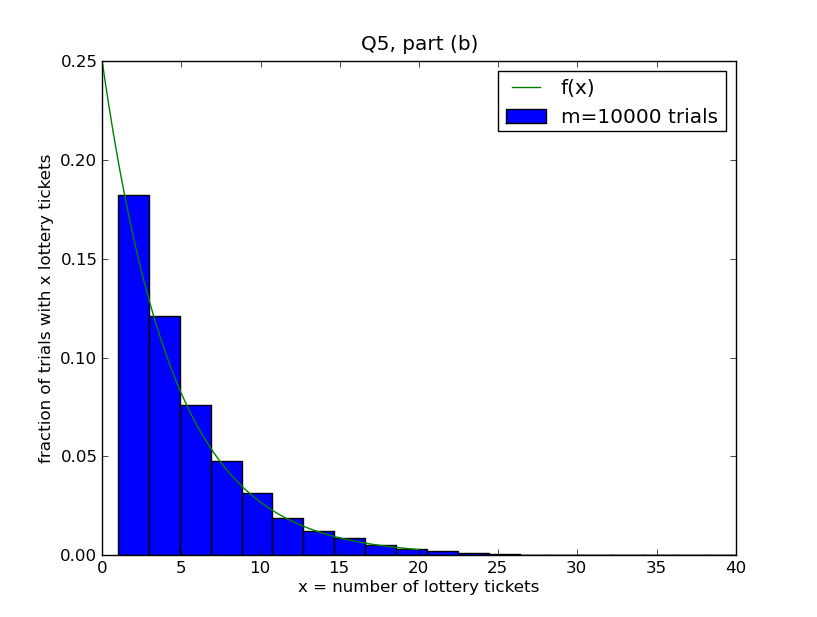
\includegraphics[width=0.5\textwidth]{part_b.png}
\end{figure}
Example average: 5.057.
}}\fi


\qpart
\item Compute $\mathbb{E}(X)$, the expected value of $X$. How does this relate to the average number of lottery tickets from part (b)? (Hint: use the relation $\mathbb{E}(X) = (1-p) \mathbb{E}(X) + 1$, but first explain where this relation comes from.)

\ifsolutions{ \answer{ 
This relation comes from the fact that with probability $p$, Lily will only need to buy 1 lottery ticket. But if she is not so lucky the first time, with probability $(1-p)$ she will have to try again.  When she tries again, her expectation from that point hasn't changed, so in a sense she is just starting over. Thus we get 1 plus the original expectation multiplied by the probability of failure on the first day:
\[ \mathbb{E}(X) = 1 + (1-p) \mathbb{E}(X). \]

Solving for $\mathbb{E}(X)$, we get
\[ \mathbb{E}(X)- (1-p)\mathbb{E}(X) = 1 \quad \Rightarrow \quad \boxed{\mathbb{E}(X) = \frac{1}{p}} \] 

This fits with our answer from part (b), since $\frac{1}{0.2} = 5$, and we got an average about about 5 days before Lily won the lottery.
}}\fi

\qpart
\item Compute the cumulative mass function (cmf) for $X$, $F(x) = \mathbb{P}(X \leq x)$.

\ifsolutions{ \answer{ 
	To compute $F(x)$ we need to add up $f(y)$, for all the $y$ less than or equal to $x$. We can use the formula for a finite geometric series:
	\[ F(x) = \sum_{y=1}^x f(x) = p \sum_{y=1}^x (1-p)^{y-1} = p \cdot \frac{1 - (1-p)^x}{1 - (1-p)} = 1 - (1-p)^x. \]
}}\fi

\qpart
\item (Optional Lab) Use your histogram from part (b) to plot an ``empirical cmf'' (i.e. for each number of tickets $x$, plot the fraction of trials where Lily bought $x$ or fewer tickets). Then overlay $F(x)$.

\ifsolutions{ \answer{
\begin{figure}[h!]
\center
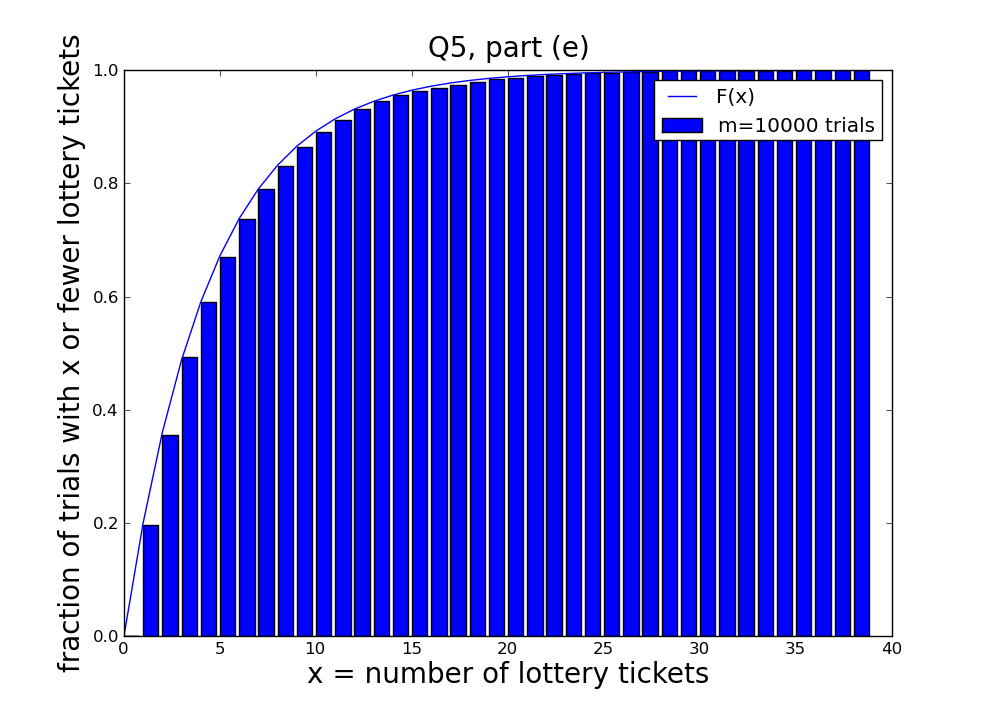
\includegraphics[width=0.5\textwidth]{part_e.png}
\end{figure}
}}\fi

\end{enumerate}





\qns{007} \\
Mr.~Bond is imprisoned in a cell from which there are three possible
ways to escape: an air-conditioning duct, a sewer pipe and the door
(which is unlocked). The air-conditioning duct leads him on a two-hour
trip whereupon he falls through a trap door onto his head, much to the
amusement of his captors. The sewer pipe is similar but takes five
hours to traverse. Each fall produces amnesia and he is returned to
the cell immediately after each fall. Assume that he always
immediately chooses one of the three exits from the cell with
probability 1/3. On the average, how long does it take before he opens
the unlocked door and escapes?

Equivalent story: A certain chainsmoker is at a party. There are
three things that she can do. She can go to the bathroom, in which
case she will take two selfies (one with a cigarette, and one
without). After this, she  again has to decide what to do. Or she can
fiddle with Instagram, in which case she will take five selfies. After
which, she again has to decide what to do. Or, she can visit her
friend Jason, at which point the party ends.  When she has to decide,
she chooses equally likely between her three choices: bathroom,
Instagram, or Jason. How many selfies will she take on average at a
party? 

[HINT: Think about how to adapt the recursive trick used to calculate
the expectation of a Geometric Random Variable to this situation. ]

%In particular, you should be able to prove that $E(T) = \frac{1}{3}E(T|A) + \frac{1}{3}E(T|S) + \frac{1}{3}E(T|D)$ 

\ifsolutions{ \answer{
Using the notation in the extremely helpful hint, $E[T]=E[T\,|\, A]\Pr[A]+E[T\,|\, S]\Pr[S]+E[T\,|\, D]\Pr[D]=\frac{1}{3}(E[T\,|\, A]+E[T\,|\, S]+E[T\,|\, D])$.
Note that $E[T\,|\, A]=E[T]+2$ by the memorylessness of the situation.
Similarly, $E[T\,|\, S]=E[T]+5$. Lastly, $E[T\,|\, D]=0$ because
Mr. Bond escapes immediately. So we have that $E[T]=\frac{1}{3}(E[T]+2+E[T]+5+0)$.
Solving this for $E[T]$, we get that $E[T]=\fbox{\ensuremath{\mathbf{007}}}$.
}}
\fi

\iffalse

\qns{(Optional) Balls and boxes}\\
Suppose $\alpha n$ balls are dropped at random into $n$ boxes so that all $n^{\alpha n}$ assignments have equal probability. Here, $n$ is large enough so that you can treat $\alpha n$ as a natural number. 
\begin{enumerate}[a)]

\qpart
\item Let $N$ be the number of empty boxes. Compute $E(N)$.
\qpart
\item If $X=N/n$ is the proportion of empty boxes, what are the limiting values of $E(X)$ as $n \rightarrow \infty$?
\qpart
\item In a real situation, given the value of $X$, how would you estimate $\alpha$ if it is unknown?
\end{enumerate}




\ifsolutions{ \answer{
\begin{itemize}
\item[a)] $Y_i=1$ if box $i$ is empty, 0 otherwise;
\[
E(N)=E(\sum_{i=1}^n Y_i)=\sum_{i=1}^n E(Y_i)=\sum_{i=1}^n P(Y_i=1)
=\sum_{i=1}^n (\frac{(n-1)^{\alpha n}}{n^{\alpha n}}) = n(1-\frac{1}{n})^{\alpha n}
\]
\item[b)] Using the fact that 
\[
\lim_{n\rightarrow \infty}(1-\frac{1}{n})^{\alpha n} = e^{\alpha}
\]

\[
E(X)=E(\frac{N}{n})=\frac{E(N)}{n}=(1-\frac{1}{n})^{\alpha n}
\]

\[\lim_{n \rightarrow \infty}E(X) = e^{\alpha} \]

\item[c)]
If $n$ is large and we know $X_n$, then our estimate of $\alpha$ would be $\hat{\alpha}=logX_n$


\end{itemize}
}}
\fi
\fi


\qns{Write your own problem} \\
Write your own problem related to this week's material and solve it. You may still work in groups to brainstorm problems, but each student should submit a unique problem. What is the problem? How to formulate it? How to solve it? What is the solution?

\qns{Midterm question 3} \\
Re-do midterm question 3.
\qns{Midterm question 4} \\
Re-do midterm question 4.
\qns{Midterm question 5} \\
Re-do midterm question 5.
\qns{Midterm question 6} \\
Re-do midterm question 6.
\qns{Midterm question 7} \\
Re-do midterm question 7.
\qns{Midterm question 8} \\
Re-do midterm question 8.
\qns{Midterm question 9} \\
Re-do midterm question 9.
\qns{Midterm question 10} \\
Re-do midterm question 10.
\qns{Midterm question 11} \\
Re-do midterm question 11.
\qns{Midterm question 12} \\
Re-do midterm question 12.
\qns{Midterm question 13} \\
Re-do midterm question 13.
\qns{Midterm question 14} \\
Re-do midterm question 14.

\end{qunlist}


%OPTIONAL PROBLEMS
%
%\begin{qunlist}
%
%\qns{Expectation Warm up}
% 
% I think it would be good to give students a warm up question on expectation. We give them a distribution, say $Pr(X = 1) = 1/2, Pr (X=2) = 1/3, Pr (x=3) = 1/6$ Then we ask them to compute the expectation.
% 
% Other warm up problems would be given the expectation, asking some questions about the probability of X. (for example, $X\geq 0, Pr(X=0) = 1/2, \mathbb{E}[X] = 10.$ True or false $Pr(X \geq 20) > 0$
%
%
%\qns{Expected number of fixed points in a permutation}
%
%It's 1, done easily through linearity of expectation
%
%
%\qns{Bubblesort} \\
%The well-known Bubblesort algorithm sorts a list $a_1, a_2, \ldots, a_n$ of numbers by repeatedly swapping adjacent numbers that are inverted (i.e., in the wrong relative order) until there are no remaining inversions. Suppose that the input to Bubblesort is a random permutation of the numbers $a_1, a_2, \ldots, a_n$, so that all $n!$ orderings are equally likely, and that all the numbers are distinct. What is the expected number of swaps performed by Bubblesort?
%
%\qns{Machine Failures} \\
%Two faulty machines, $M_1$ and $M_2$, are repeatedly run synchronously in parallel (i.e., both machines execute one run, then both execute a second run, and so on). On each run, $M_1$ fails with probability $p_1$ and $M_2$ with probability $p_2$, all failure events being independent. Let the random variables $X_1$, $X_2$ denote the number of runs until the first failure of $M_1$, $M_2$ respectively; thus $X_1$, $X_2$ have geometric distributions with parameters $p_1$, $p_2$ respectively.
%Let $X$ denote the number of runs until the first failure of either machine. Show that $X$ also has a geometric distribution, with parameter $p_1 + p_2 − p_1p_2.$
%
%\qns{St. Petersburg Paradox}
%
%Consider a single-player game where the pot initially contains \$1. Then a fair coin is tossed until it comes up tails, at which point the player gets all the money in the pot. Each time a head comes up, the amount of money in the pot is doubled.  So if a tails comes up first, the player gets \$1.  If the first tails comes up second, the player gets \$2, if tails comes up third, the player gets \$4, and so on.
%
%\begin{enumerate}[a)]
%
%\qpart
%\item For $m=1,2,3, \cdots 1,000$, simulated $m$ trials of this game.  For each $m$, compute the average winnings of the player.  Plot the average winnings on the $y$-axis vs. $m$ on the $x$-axis.  What do you notice?  Are the average winnings converging to a specific value?
%
%\qpart
%\item Now compute the expected value of the winnings.  How can you reconcile this result with part (a)?
%\end{enumerate}
%

%\qns{Problem from Chung-Wei} \\
%TODO get figs from Chung-Wei if you use this problem
%There are $n$ vertices $\{v_1,v_2,\ldots,v_n\}$ on a plane, and the coordinates of $v_i$ are $(x_i,y_i)$. The bounding box of $v_i$ and $v_j$ is a rectangular $\{(x,y)|(x-x_i)(x-x_j)\leq 0\mbox{ and }(y-y_i)(y-y_j)\leq 0\}$. An edge is added between two vertices if and only if there is no other vertex inside or on the boundary of the bounding box of the two vertices. Prove that the expected number of edges is smaller than $(2n+2)\ln n$.
%
%\ifsolutions{ \answer{
%The number of edges in the OASG is $O(n^2)$ in the worst case, but Theorem~\ref{theorem:edge-random-case} shows that the expected number of edges in the OASG is $O(n\lg n)$. To compute the expected number of edges in the OASG, several notations and lemmas are first given.
%
%\begin{Definition}\label{def:g1}
%Given an instance, $G_1:(V_1,E_1)$ is defined as the OASG.
%\end{Definition}
%
%\begin{Definition}\label{def:g2}
%Given an instance, $G_2:(V_2,E_2)$ is defined as the OASG constructed after regarding all corner-vertices as pin-vertices and removing all obstacles from the plane, \emph{i.e.}, there are totally $n$ pin-vertices and no obstacle on the plane.
%\end{Definition}
%
%\begin{Definition}\label{def:g3}
%Given an instance, $G_3:(V_3,E_3)$ is defined as the OASG constructed after regarding all corner-vertices as pin-vertices, removing all obstacles from the plane, and moving a small enough distance, $\varepsilon$, for vertices with the same $x$-coordinate or $y$-coordinate so that all vertices have different $x$-coordinates and $y$-coordinates.
%\end{Definition}
%
%%\begin{figure}
%%\centering
%%\psfig{figure=nlogn-proof1.eps,width=12cm}
%%\caption{\small An example of $G_1$, $G_2$, and $G_3$. (a) Given an instance, (b) $G_1$ has fewer edges than (c) $G_2$ which has fewer edges than (d) $G_3$.} \label{fig:nlogn-proof1}
%%\end{figure}
%
%See Figure~\ref{fig:nlogn-proof1} for an example of $G_1$, $G_2$, and $G_3$.
%
%\begin{Definition}\label{def:gamma}
%Given an instance, a permutation $\Gamma$ is defined by labelling from 1 to $n$ for the vertices in $G_3$ by the order of their $y$-coordinates and permuting these labelled numbers by the order of their $x$-coordinates.
%\end{Definition}
%
%\begin{Definition}\label{def:n4}
%Given a permutation $\Gamma$, $N_4$ is defined as the number of pairs $(i,j)$, where $1\leq i,j\leq n$, and there is no integer whose value is between $i$ and $j$ and whose position in the permutation $\Gamma$ is between the positions of $i$ and $j$.
%\end{Definition}
%
%%\begin{figure}
%%\centering
%%\psfig{figure=nlogn-proof2.eps,width=12cm}
%%\caption{\small (a) Given the $G_3$, $\Gamma$ is defined by (b) labelling from 1 to $n$ for vertices in $G_3$ by the order of their $y$-coordinates and (c) permuting these labelled numbers by the order of their $x$-coordinates, resulting in $\Gamma=<2,1,3,5,4>$. (d) The six pairs make $N_4=6$ which is equal to the number of edges in $G_3$.} \label{fig:nlogn-proof2}
%%\end{figure}
%
%%See Figure~\ref{fig:nlogn-proof2} for an example of the permutation $\Gamma$ and $N_4$. There are the following lemmas.
%
%\begin{Lemma}\label{lemma:e1-e2}
%$|E_1|\leq |E_2|$.
%\end{Lemma}
%
%\begin{Proof}
%For any edge in $G_1$, it is always in $G_2$, but there are some edges in $G_2$ whose corresponding edges in $G_1$ are blocked by obstacles. As a result, $|E_1|\leq |E_2|$.
%\end{Proof}
%
%\begin{Lemma}\label{lemma:e2-e3}
%$|E_2|\leq |E_3|$.
%\end{Lemma}
%
%\begin{Proof}
%For any edge $(v_1,v_2)$ in $G_2$, there is no other vertex inside or on the boundary of the bounding box of $v_1$ and $v_2$. Because the moving of each vertex is small enough, there is still no other vertex inside or on the boundary of the bounding box of $v_1$ and $v_2$. As a result, $(v_1,v_2)$ is still in $G_3$, and $|E_2|\leq |E_3|$.
%\end{Proof}
%
%\begin{Lemma}\label{lemma:e3-n4}
%$|E_3|=N_4$.
%\end{Lemma}
%
%\begin{Proof}
%For vertices $v_1$, $v_2$, and $v_3$ in $G_3$, the $y$-coordinate of $v_3$ is between those of $v_1$ and $v_2$ if and only if its labelled number is between those of $v_1$ and $v_2$; the $x$-coordinate of $v_3$ is between those of $v_1$ and $v_2$ if and only if its position in the permutation $\Gamma$ is between those of $v_1$ and $v_2$. For any edge $(v_1,v_2)$ in $G_3$, there is no other vertex inside or on the boundary of the bounding box of $v_1$ and $v_2$, resulting in a pair of $(i,j)$ in $\Gamma$ where there is no integer whose value is between $i$ and $j$ and whose position in $\Gamma$ is between those of $i$ and $j$. On the other hand, a pair of $(i,j)$ in $\Gamma$ where there is no integer whose value is between $i$ and $j$ and whose position in $\Gamma$ is between those of $i$ and $j$ means that there is no other vertex inside or on the boundary of the bounding box of the two corresponding vertices. As a result, $|E_3|=N_4$ due to the one-to-one mapping.
%\end{Proof}
%
%\begin{Lemma}\label{lemma:n4}
%The expected value of $N_4$ is $O(n\lg n)$.
%\end{Lemma}
%
%\begin{Proof}
%For any pair $(i,i+j)$ where $i\geq 1$, $j\geq 1$, and $i+j\leq n$, there are $(j+1)!$ permutations from $i$ to $i+j$. Among these $(j+1)!$ permutations, $(i,i+j)$ is counted if and only if $i$ and $i+j$ are permuted successively; otherwise, there is at least an integer between $i$ and $i+j$ whose position in $\Gamma$ is between positions of $i$ and $j$. Because there are $2j!$ permutations from $i$ to $i+j$ where $i$ and $i+j$ are permuted successively, and there are $n!$ permutation from 1 to $n$, the pair $(i,i+j)$ is counted $n!\frac{2j!}{(j+1)!}$ times among all permutations from 1 to $n$.
%
%Because there are $(n-j)$ types of pairs $(i,i+j)$, the total count is $\sum_{j=1}^{n-1}((n-j)n!\frac{2j!}{(j+1)!})$ among all permutations from 1 to $n$. Therefore, the expected value of $N_4$ is
%\begin{eqnarray*}
% & {\textstyle        } & {\textstyle \frac{1}{n!}\sum_{j=1}^{n-1}\left((n-j)n!\frac{2j!}{(j+1)!}\right)}            \nonumber\\
% & {\textstyle { }={ }} & {\textstyle \sum_{j=1}^{n-1}\left((n-j)\frac{2}{j+1}\right)}                               \nonumber\\
%%& {\textstyle { }={ }} & {\textstyle 2\sum_{j=1}^{n-1}\left(\frac{n}{j+1}-\frac{j}{j+1}\right)}                     \nonumber\\
% & {\textstyle { }={ }} & {\textstyle 2n\sum_{j=1}^{n-1}\frac{1}{j+1}-2\sum_{j=1}^{n-1}\left(1-\frac{1}{j+1}\right)} \nonumber\\
% & {\textstyle { }={ }} & {\textstyle (2n+2)\sum_{j=1}^{n-1}\frac{1}{j+1}-2(n-1)}                                    \nonumber\\
% & {\textstyle { }<{ }} & {\textstyle (2n+2)\int_1^n\left(\frac{1}{x}\right)dx-2(n-1)}                             \nonumber\\
% & {\textstyle { }={ }} & {\textstyle (2n+2)\ln n-2(n-1)}                                                           \nonumber
%\end{eqnarray*}
%As a result, the expected value of $N_4$ is $O(n\lg n)$.
%\end{Proof}
%
%\begin{Theorem}\label{theorem:edge-random-case}
%The expected number of edges in the OASG is $O(n\lg n)$.
%\end{Theorem}
%
%\begin{Proof}
%Given an instance, by Lemmas~\ref{lemma:e1-e2}, \ref{lemma:e2-e3}, and \ref{lemma:e3-n4}, the number of edges in the OASG is less than its corresponding $N_4$. By Lemma~\ref{lemma:n4}, the expected value of $N_4$ is $O(n\lg n)$. As a result, the expected number of edges in the OASG is $O(n\lg n)$ since the probability for each kind of the permutation $\Gamma$ is the same.
%\end{Proof}
%}} \fi
%    
%\end{qunlist}

\end{document}
